\section{Messprotokolle}

%Kalibrierung
\begin{figure}[!ht]
 \centering
 \includegraphics[width=0.8\textwidth]{fig/Messprotokolle/Kalibrierung.png}
 \caption{Messprotokoll zur Kalibrierungsmessung}
 \label{fig:MPKalibrierung}
\end{figure}

%Vergleich
\begin{figure}[!ht]
 \centering
 \includegraphics[width=\textwidth]{fig/Messprotokolle/VergleichMagnetometer.png}
 \caption{Messprotokoll zum Vergleich der Protonenmagnetometer und des Fluxgates}
 \label{fig:MPVergleich}
\end{figure}

%Huette
\begin{figure}[!ht]
 \centering
 \includegraphics[width=\textwidth]{fig/Messprotokolle/EinflussHuette.png}
 \caption{Messprotokoll zum Profil zur Untersuchung der Einflüsse äußerer Störfaktoren auf die Basismessung}
 \label{fig:MPHuette}
\end{figure}

\FloatBarrier
\section{Sonstige Abbildungen} %???Anderer Name

\begin{figure}[!ht]
 \centering
 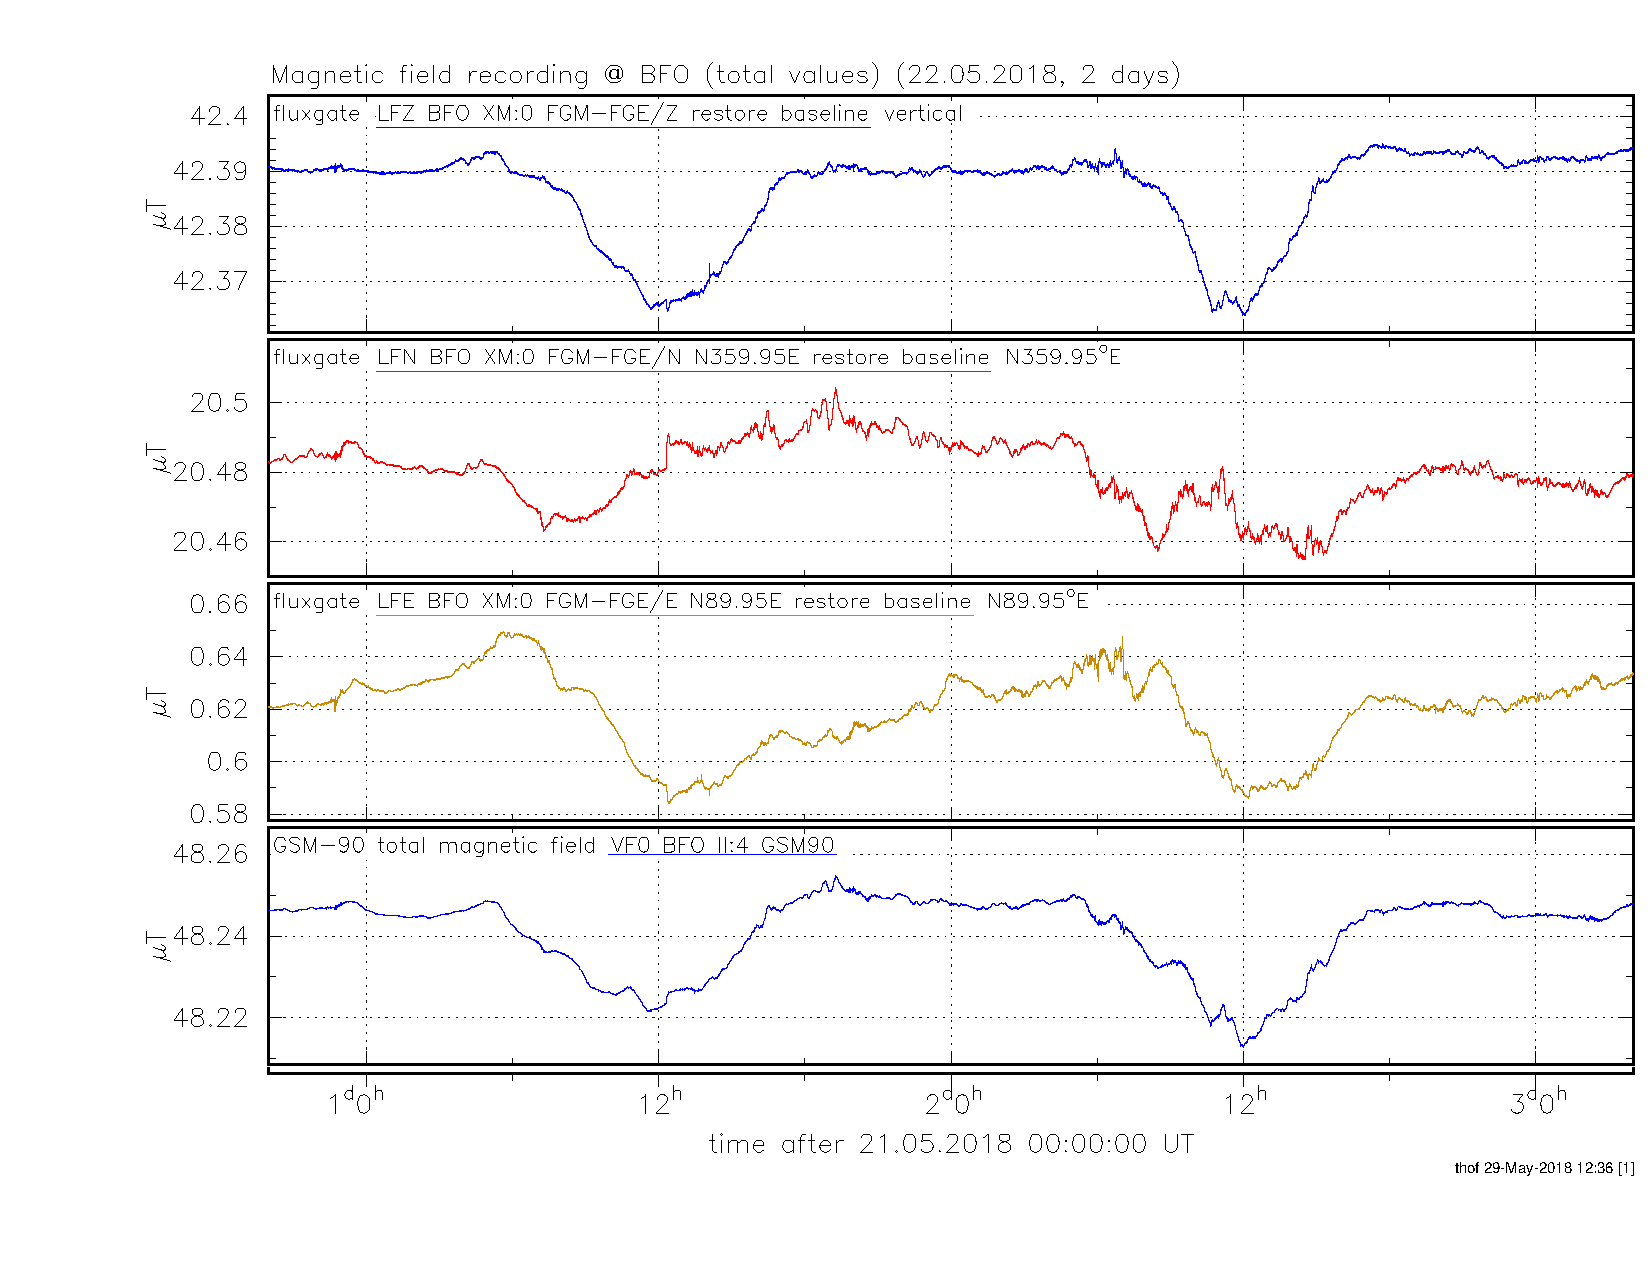
\includegraphics[width=\textwidth]{fig/Magnetfeld_BFO_2_Tage.pdf}
 \caption[Messung des Magnetfelds am BFO]{Messung des Magnetfelds am BFO. Von oben nach unten: Vertikalkomponente, Nordkomponente und Ostkomponente mit einem Fluxgate gemessen, Totalintensität mit einem Overhauser-Magnetometer gemessen}
 \label{fig:BFO}
\end{figure}

% \begin{figure}[h!]
%  \centering
%  \includegraphics[width=\textwidth]{fig/Messprotokolle/}
%  \caption{}
%  \label{fig:}
% \end{figure}